\documentclass{scrartcl}
\usepackage[margin=3cm]{geometry}
\usepackage{amsmath}
\usepackage{amssymb}
\usepackage{amsthm}
\usepackage{blindtext}
\usepackage{datetime}
\usepackage{fontspec}
\usepackage{float}
\usepackage{graphicx}
\usepackage{kotex}
\usepackage[lighttt]{lmodern}
\usepackage{listings}
\usepackage{mathrsfs}
\usepackage{mathtools}
\usepackage{pgf,tikz,pgfplots}

\pgfplotsset{compat=1.15}
\usetikzlibrary{arrows}
\newtheorem{theorem}{Theorem}

\lstset{
  numbers=none, frame=single, showspaces=false, showstringspaces=false,
  showtabs=false, breaklines=true, showlines=true, breakatwhitespace=true,
  basicstyle=\ttfamily, keywordstyle=\bfseries, basewidth=0.5em
}

\setmainhangulfont{Noto Serif CJK KR}[
  UprightFont=* Light, BoldFont=* Bold,
  Script=Hangul, Language=Korean, AutoFakeSlant,
]
\setsanshangulfont{Noto Sans CJK KR}[
  UprightFont=* DemiLight, BoldFont=* Medium,
  Script=Hangul, Language=Korean
]
\setmathhangulfont{Noto Sans CJK KR}[
  SizeFeatures={
    {Size=-6,  Font=* Medium},
    {Size=6-9, Font=*},
    {Size=9-,  Font=* DemiLight},
  },
  Script=Hangul, Language=Korean
]
\title{CSED353: Chap. 2 Exercises (due Mar. 18)}
\author{손량(20220323)}
\date{Last compiled on: \today, \currenttime}

\newcommand{\un}[1]{\ensuremath{\ \mathrm{#1}}}

\begin{document}
\maketitle

\section{Problem \#1}

\subsection{Solution for (a)}
From the parameters given in the question, we can determine the parameters for
internet access link as follows:
\begin{align*}
  L = 2,000,000 \un{bits/req} \quad
  R = 54,000,000 \un{bps} \quad
  a = 20 \un{req/s}
\end{align*}
Then, the utilization for access link is
\begin{align*}
  \rho = \frac{La}{R} = 0.741
\end{align*}
So the access link delay can be calculated as
\begin{align*}
  \frac{L}{R} \left( \frac{\rho}{1 - \rho} \right) + \frac{L}{R}
  = 0.143 \un{s}
\end{align*}
For LAN, we can use \(R = 10,000,000,000 \un{bps}\) and obtain the LAN
utilization of
\begin{align*}
  \rho = \frac{La}{R} = 0.004
\end{align*}
so the LAN delay can be calculated as
\begin{align*}
  \frac{L}{R} \left( \frac{\rho}{1 - \rho} \right) + \frac{L}{R}
  = 0.000201 \un{s}
\end{align*}
Since the internet delay is given as 3 seconds, we obtain the final result as
\begin{align*}
  0.143 \un{s} + 3 \un{s} + 0.000201 \un{s} = 3.143 \un{s}
\end{align*}

\subsection{Solution for (b)}
By taking cache into account, we can obtain utilization for access link as
\begin{align*} 
  \rho = 0.4 \times \frac{La}{R} = 0.296
\end{align*}
Assuming that round trip from and to the local web cache is negligible in the
case of cache miss, the delay from the origin servers can be obtained as
\begin{align*}
  \frac{L}{R} \left( \frac{\rho}{1 - \rho} \right) + \frac{L}{R} + 3 \un{s}
  = 3.05 \un{s}
\end{align*}
The utilization of LAN is
\begin{align*}
  \rho = 0.6 \times \frac{La}{R} = 0.0240
\end{align*}
Then the delay for cache server can be obtained as
\begin{align*}
  \frac{L}{R} \left( \frac{\rho}{1 - \rho} \right) + \frac{L}{R}
  = 0.00205 \un{s}
\end{align*}
The final result is
\begin{align*}
  0.4 \times 3.05 \un{s} + 0.6 \times 0.00205 \un{s} = 1.22 \un{s}
\end{align*}

\section{Problem \#2}

\subsection{Solution for (a)}
The numbers of fields in question are as follows:

\begin{itemize}
  \item Questions: 1
  \item Answer RRs: 0
  \item Authority RRs: 0
  \item Additional RRs: 0
\end{itemize}

Question section has information about the query being made. There is one
question field in the captured packet, which is a question asking for the
address of \texttt{cse.postech.ac.kr}. Answer RRs are answers for given
question. RR is an acronym for ``request record''. Since this packet is a
packet sent from the client to the server, there is no data for this section.
Authority RRs contains records for other authoritative servers, and additional
RRs has other helpful records. Like answer RRs, these fields typically contin
answers from DNS servers, so there is no data for these sections as well.

\subsection{Solution for (b)}
\begin{figure}[H]
\centering
\begin{tabular}{|l|lllll|}
\hline
 & \multicolumn{1}{l|}{Name} & \multicolumn{1}{l|}{Type} & \multicolumn{1}{l|}{Address} & \multicolumn{1}{l|}{Name server} & Time to live \\ \hline
Answers & \multicolumn{1}{l|}{cse.postech.ac.kr} & \multicolumn{1}{l|}{A} & \multicolumn{1}{l|}{141.223.5.78} & \multicolumn{1}{l|}{} & 172800 \\ \hline
\begin{tabular}[c]{@{}l@{}}Authoritative\\ nameservers\end{tabular} & \multicolumn{5}{c|}{N/A} \\ \hline
\begin{tabular}[c]{@{}l@{}}Additional\\ records\end{tabular} & \multicolumn{5}{c|}{N/A} \\ \hline
\end{tabular}
\end{figure}

\subsection{Solution for (c)}
No authoritative servers were listed in the captured packet.

\subsection{Solution for (d)}
SOA record is a record which has administrative information about the zone.

\subsection{Solution for (e)}
The response packet contains this RR because we queried nonexistent domain.
Since there is no address corresponding to the domain, the DNS system instead
responds with information about the zone corresponding to \texttt{ac.kr}. In
our situation, we deliberately picked such domain so the provided information
in SOA record is of no use. However, if we are really wanting the address for
this domain and there was none found, the information in the record might be
useful for troubleshooting and debugging.

\subsection{Solution for (f)}
We can infer that the DNS queries of the two examples were recursive as the DNS
server responded immediately with answer or authoritative nameservers.

\section{Problem \#3}

\subsection{Solution for (a)}
Two packets were captured:

\begin{figure}[H]
  \centering
  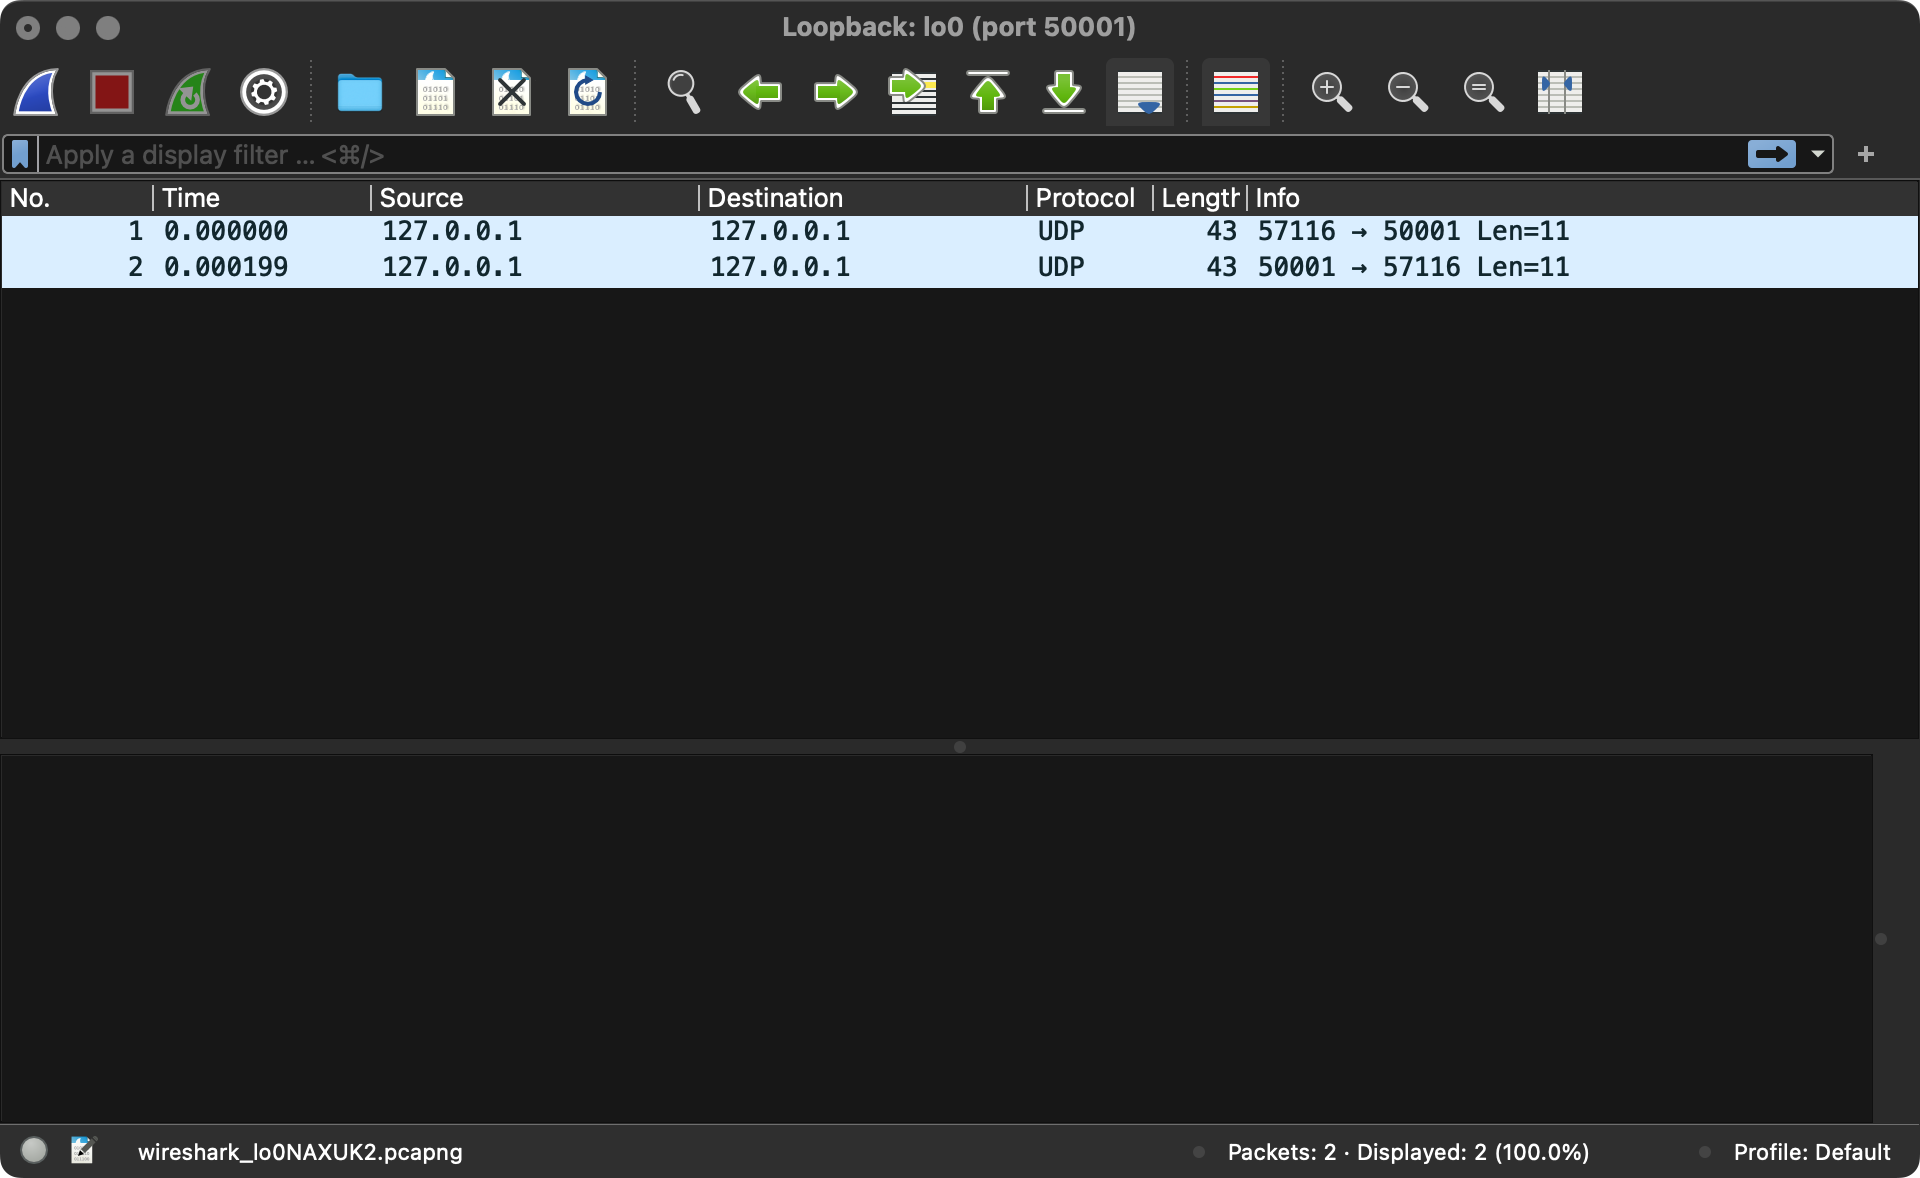
\includegraphics[width=0.8\linewidth]{prob3a}
\end{figure}

\subsection{Solution for (b)}
One packet(the first one) was sent from the client to the server, and the
another one(the second one) was sent from the server to the client. The client
used port 57116 to communicate with the server.

\begin{figure}[H]
\begin{tabular}{|l|l|l|l|l|l|l|l|}
\hline
\begin{tabular}[c]{@{}l@{}}Packet\\ No.\end{tabular} & \begin{tabular}[c]{@{}l@{}}Src.\\ IP\end{tabular} & \begin{tabular}[c]{@{}l@{}}Src.\\ Port\end{tabular} & \begin{tabular}[c]{@{}l@{}}Dest.\\ IP\end{tabular} & \begin{tabular}[c]{@{}l@{}}Dest.\\ Port\end{tabular} & \begin{tabular}[c]{@{}l@{}}Data\\ Length\end{tabular} & Data & \begin{tabular}[c]{@{}l@{}}Text-converted\\ Data\end{tabular} \\ \hline
N/A &  &  &  &  &  &  &  \\ \hline
\multicolumn{8}{|c|}{bp1} \\ \hline
1 & 127.0.0.1 & 60783 & 127.0.0.1 & 50001 & 11 & \texttt{68656c6c20776f726c6421} & \texttt{hell world!} \\ \hline
\multicolumn{8}{|c|}{bp2} \\ \hline
2 & 127.0.0.1 & 50001 & 127.0.0.1 & 60783 & 11 & \texttt{48454c4c20574f524c4421} & \texttt{HELL WORLD!} \\ \hline
\end{tabular}
\end{figure}

\section{Problem \#4}

\subsection{Solution for (a)}
12 packets were captured:

\begin{figure}[H]
  \centering
  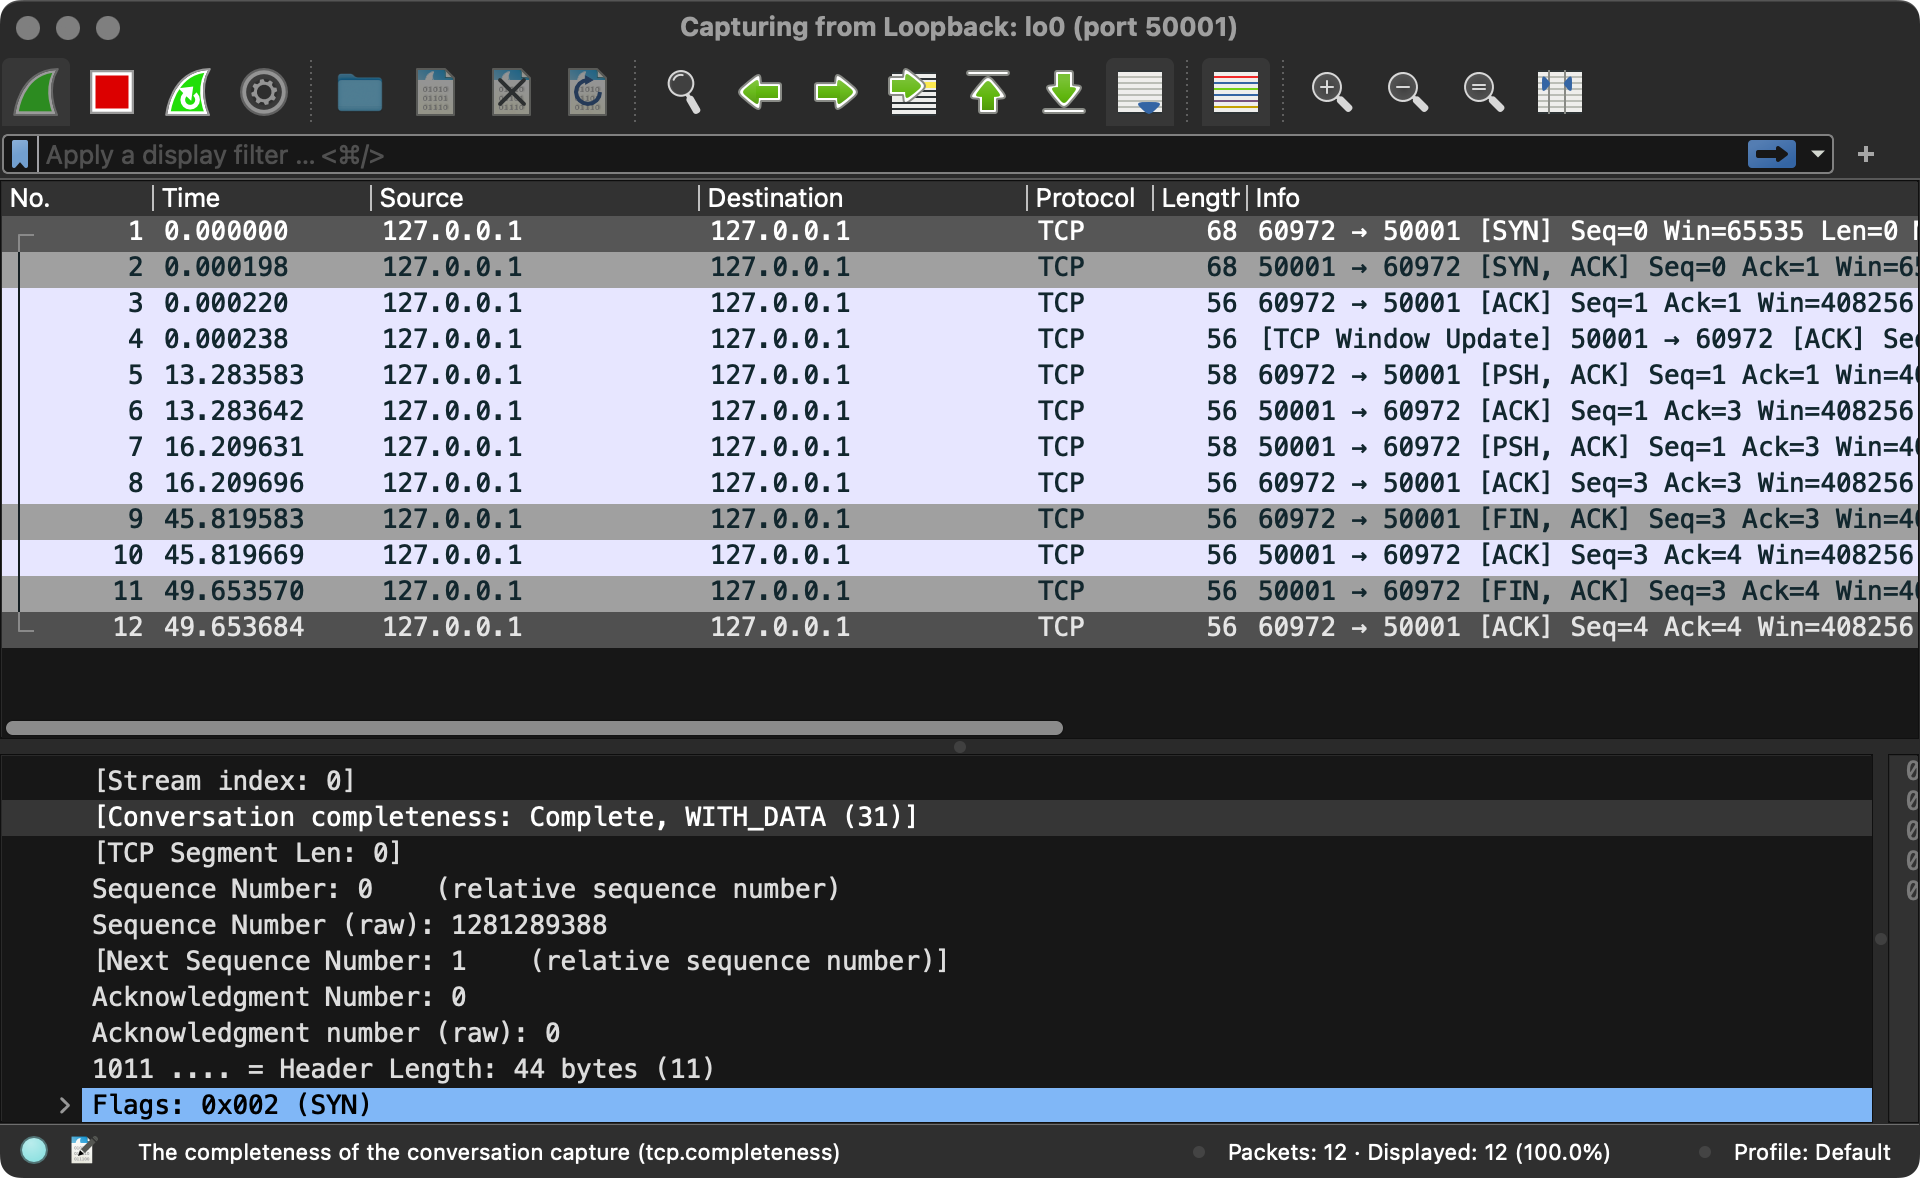
\includegraphics[width=0.8\linewidth]{prob4a}
\end{figure}

Compared to the UDP exercise, 10 more packets were captured.

\subsection{Solution for (b)}
Six packets were sent from the client to the server, and the other six were
from the server to the client. The client used port 60972 to communicate with
the server.

\begin{figure}[H]
\begin{tabular}{|lllllllll|}
\hline
\multicolumn{1}{|l|}{\begin{tabular}[c]{@{}l@{}}Packet\\ No.\end{tabular}} & \multicolumn{1}{l|}{\begin{tabular}[c]{@{}l@{}}Source\\ IP\end{tabular}} & \multicolumn{1}{l|}{\begin{tabular}[c]{@{}l@{}}Source\\ Port\end{tabular}} & \multicolumn{1}{l|}{\begin{tabular}[c]{@{}l@{}}Dest.\\ IP\end{tabular}} & \multicolumn{1}{l|}{\begin{tabular}[c]{@{}l@{}}Dest.\\ Port\end{tabular}} & \multicolumn{1}{l|}{Flags} & \multicolumn{1}{l|}{\begin{tabular}[c]{@{}l@{}}Data\\ Length\end{tabular}} & \multicolumn{1}{l|}{Data} & \begin{tabular}[c]{@{}l@{}}Text-converted\\ Data\end{tabular} \\ \hline
\multicolumn{1}{|l|}{N/A} & \multicolumn{1}{l|}{} & \multicolumn{1}{l|}{} & \multicolumn{1}{l|}{} & \multicolumn{1}{l|}{} & \multicolumn{1}{l|}{} & \multicolumn{1}{l|}{} & \multicolumn{1}{l|}{} &  \\ \hline
\multicolumn{9}{|c|}{bp1} \\ \hline
\multicolumn{1}{|l|}{1} & \multicolumn{1}{l|}{127.0.0.1} & \multicolumn{1}{l|}{60972} & \multicolumn{1}{l|}{127.0.0.1} & \multicolumn{1}{l|}{50001} & \multicolumn{1}{l|}{SYN} & \multicolumn{1}{l|}{} & \multicolumn{1}{l|}{} &  \\ \hline
\multicolumn{1}{|l|}{2} & \multicolumn{1}{l|}{127.0.0.1} & \multicolumn{1}{l|}{50001} & \multicolumn{1}{l|}{127.0.0.1} & \multicolumn{1}{l|}{60972} & \multicolumn{1}{l|}{SYN, ACK} & \multicolumn{1}{l|}{} & \multicolumn{1}{l|}{} &  \\ \hline
\multicolumn{1}{|l|}{3} & \multicolumn{1}{l|}{127.0.0.1} & \multicolumn{1}{l|}{60972} & \multicolumn{1}{l|}{127.0.0.1} & \multicolumn{1}{l|}{50001} & \multicolumn{1}{l|}{ACK} & \multicolumn{1}{l|}{} & \multicolumn{1}{l|}{} &  \\ \hline
\multicolumn{1}{|l|}{4} & \multicolumn{1}{l|}{127.0.0.1} & \multicolumn{1}{l|}{50001} & \multicolumn{1}{l|}{127.0.0.1} & \multicolumn{1}{l|}{60972} & \multicolumn{1}{l|}{ACK} & \multicolumn{1}{l|}{} & \multicolumn{1}{l|}{} &  \\ \hline
\multicolumn{9}{|c|}{bp2} \\ \hline
\multicolumn{1}{|l|}{5} & \multicolumn{1}{l|}{127.0.0.1} & \multicolumn{1}{l|}{60972} & \multicolumn{1}{l|}{127.0.0.1} & \multicolumn{1}{l|}{50001} & \multicolumn{1}{l|}{PSH, ACK} & \multicolumn{1}{l|}{2} & \multicolumn{1}{l|}{\texttt{6869}} & \texttt{hi} \\ \hline
\multicolumn{1}{|l|}{6} & \multicolumn{1}{l|}{127.0.0.1} & \multicolumn{1}{l|}{50001} & \multicolumn{1}{l|}{127.0.0.1} & \multicolumn{1}{l|}{60972} & \multicolumn{1}{l|}{ACK} & \multicolumn{1}{l|}{} & \multicolumn{1}{l|}{} &  \\ \hline
\multicolumn{9}{|c|}{bp3} \\ \hline
\multicolumn{1}{|l|}{7} & \multicolumn{1}{l|}{127.0.0.1} & \multicolumn{1}{l|}{50001} & \multicolumn{1}{l|}{127.0.0.1} & \multicolumn{1}{l|}{60972} & \multicolumn{1}{l|}{PSH, ACK} & \multicolumn{1}{l|}{2} & \multicolumn{1}{l|}{\texttt{4849}} & \texttt{HI} \\ \hline
\multicolumn{1}{|l|}{8} & \multicolumn{1}{l|}{127.0.0.1} & \multicolumn{1}{l|}{60972} & \multicolumn{1}{l|}{127.0.0.1} & \multicolumn{1}{l|}{50001} & \multicolumn{1}{l|}{ACK} & \multicolumn{1}{l|}{} & \multicolumn{1}{l|}{} &  \\ \hline
\multicolumn{9}{|c|}{bp4} \\ \hline
\multicolumn{1}{|l|}{9} & \multicolumn{1}{l|}{127.0.0.1} & \multicolumn{1}{l|}{60972} & \multicolumn{1}{l|}{127.0.0.1} & \multicolumn{1}{l|}{50001} & \multicolumn{1}{l|}{FIN, ACK} & \multicolumn{1}{l|}{} & \multicolumn{1}{l|}{} &  \\ \hline
\multicolumn{1}{|l|}{10} & \multicolumn{1}{l|}{127.0.0.1} & \multicolumn{1}{l|}{50001} & \multicolumn{1}{l|}{127.0.0.1} & \multicolumn{1}{l|}{60972} & \multicolumn{1}{l|}{ACK} & \multicolumn{1}{l|}{} & \multicolumn{1}{l|}{} &  \\ \hline
\multicolumn{9}{|c|}{bp5} \\ \hline
\multicolumn{1}{|l|}{11} & \multicolumn{1}{l|}{127.0.0.1} & \multicolumn{1}{l|}{50001} & \multicolumn{1}{l|}{127.0.0.1} & \multicolumn{1}{l|}{60972} & \multicolumn{1}{l|}{FIN, ACK} & \multicolumn{1}{l|}{} & \multicolumn{1}{l|}{} &  \\ \hline
\multicolumn{1}{|l|}{12} & \multicolumn{1}{l|}{127.0.0.1} & \multicolumn{1}{l|}{60972} & \multicolumn{1}{l|}{127.0.0.1} & \multicolumn{1}{l|}{50001} & \multicolumn{1}{l|}{ACK} & \multicolumn{1}{l|}{} & \multicolumn{1}{l|}{} &  \\ \hline
\end{tabular}
\end{figure}

\end{document}
% vim: textwidth=79
